\documentclass{article}
\usepackage{listings}
\usepackage{color}
\usepackage{float}
\usepackage{graphicx}

\definecolor{dkgreen}{rgb}{0,0.6,0}
\definecolor{gray}{rgb}{0.5,0.5,0.5}
\definecolor{mauve}{rgb}{0.58,0,0.82}

\lstset{
	frame=single,
	language=C,
	belowskip=3mm,
	showstringspaces=false,
	columns=flexible,
	captionpos=b,
	basicstyle={\small\ttfamily},
	numbers=left,
	numbersep=5pt,
	%numbers=none,
	numberstyle=\tiny\color{gray},
	keywordstyle=\color{blue},
	commentstyle=\color{dkgreen},
	stringstyle=\color{mauve},
	breaklines=true,
	breakatwhitespace=true,
	tabsize=4
}

\input kvmacros
\sloppy
\begin{document}

\title{Project 3: Memory Management}
\author{\textit{Yesheng Ma}}
\date{\today}
{\bf\small CS353: Linux Kernel}\hfill{\bf\small 2017 Spring}
{\let\newpage\relax\maketitle}
\maketitle


\begin{abstract}
In this project, we are going to look into the Linux memory management system and try to write a kernel module that deals with virtual memory address translation.
\end{abstract}


\section{Introduction}
In this project, we will mainly deal with memory management and we will interact with Linux kernel by a Linux kernel model. This module will create a file \texttt{/proc/mtest} and should meet the following requirements:
\begin{itemize}
\item listvma: list all the virtual memory area of this process.
\item findpage vm: print the physical address related to the input virtual address.
\item writeval vm val: write a unsigned long integer to a virtual memory address.
\end{itemize}

\section{Create proc File}
As what we have done in previous projects, we should first create a file under proc file system. The core kernel API we use is \verb|proc_create| where a \texttt{file\_operations} should be specified.

The module initialization part is listed as follows:
\begin{lstlisting}[language=C]
static int __init mtest_init(void)
{
	struct proc_dir_entry *entry;

	printk(KERN_INFO "mtest installed\n");
	entry = proc_create("mtest", 0666, NULL, &mtest_fops);
	if (!entry)
		return -1;
	return 0;
}
\end{lstlisting}
where the most important part is the file operations struct \verb|mtest_init|:
\begin{lstlisting}
static struct file_operations mtest_fops =
{
	.owner		= THIS_MODULE,
	.open		= mtest_open,
	.read		= seq_read,
	.write		= mtest_write,
	.llseek		= seq_lseek,
	.release	= single_release,
};
\end{lstlisting}

\section{Core Implementation}
The core implementation of this project is within the function \verb|mtest_write|. This function mainly deals with three kinds of inputs and further use some helper functions to interact to kernel. The code is shown as follows:
\begin{lstlisting}[language=C]
if (memcmp(cmd, "findpage", 8)) {
	list_vma();
} else if (memcmp(cmd, "findpage", 8) == 0) {
	if (sscanf(cmd+8, "%lx", &v1) == 1)
		find_page(v1);
} else if (memcmp(cmd, "writeval", 8) == 0) {
	if (sscanf(cmd+8, "%lx %lx", &v1, &v2) == 2)
		write_val(v1, v2);
} else {
	printk(KERN_INFO "Invalid input\n");
}
\end{lstlisting}
And next we will analyze how to implement the core functions \verb|list_vma|, \verb|find_page|, and \verb|write_val|.
\subsection{List VMA}
List virtual memory area is quite easy. The task struct of current process can be easily access by \texttt{current} macro and we can easily get the memory map by \texttt{current->mm->mmap}, the code is shown as follows:
\begin{lstlisting}[language=c]
down_read(&mm->mmap_sem);
for (vma = mm->mmap; vma; vma = vma->vm_next) {
	if (vma->vm_flags & VM_READ) a[0] = 'r';
	else a[0] = '-';
	if (vma->vm_flags & VM_WRITE) a[1] = 'w';
	else a[1] = '-';
	if (vma->vm_flags & VM_EXEC) a[2] = 'x';
	else a[2] = '-';
	printk("0x%lx 0x%lx %c%c%c\n", vma->vm_start, vma->vm_end, a[0], a[1], a[2]);
}
\end{lstlisting}
Do remember to hold the lock for memory map here.

\subsection{Find page}
To find the physical address of a virtual address, we first need to get the translation of the page of the virtual address. First, we can find the virtual memory area of this virtual address by \verb|find_vma(vma, addr)| and we will get a \verb|vm_area_struct| and the page directory is stored in \verb|vma->mm|.

Next we will walk into this page table to figure out the translated address. The first level is page global directory(pgd), the second level is page upper directory, the third level is page middle directory and the last level is page table entry. After we figure out the page table entry, i.e.\ page frame number, we can get the page related to it using \verb|pfn_to_page|. Then we can get the page address of this page using \verb|page_address| and by concatnating its latter bits, we can get the page's physical address. The code is shown as follows:
\begin{lstlisting}[language=c]
// seek page table entry
pgd = pgd_offset(mm, addr);
pud = pud_offset(pgd, addr);
pmd = pmd_offset(pud, addr);
pte = pte_offset_map(mm, pmd, addr, &ptl);
page = pfn_to_page(pte_pfn(*pte));
get_page(page);

// get physical address from page info
kern_addr = (unsigned long) page_address(page);
kern_addr += (addr & ~PAGE_MASK);
\end{lstlisting}

\subsection{Write Value}
With the help of last question, this one is easier to solve: to directly write to that memory location if that address is writable. The code is shown as follows:
\begin{lstlisting}[language=C]
// check for permission
if (!(vma->vm_flags & VM_WRITE))
	...

// write to that location
kern_addr = (unsigned long) page_address(page);
kern_addr += addr & ~PAGE_MASK;
*(unsigned long *) kern_addr = val;
\end{lstlisting}



\section{Experiment}
I tested the kernel model on Arch Linux virtual machine and here are the results.
\begin{figure}[H]
\centering
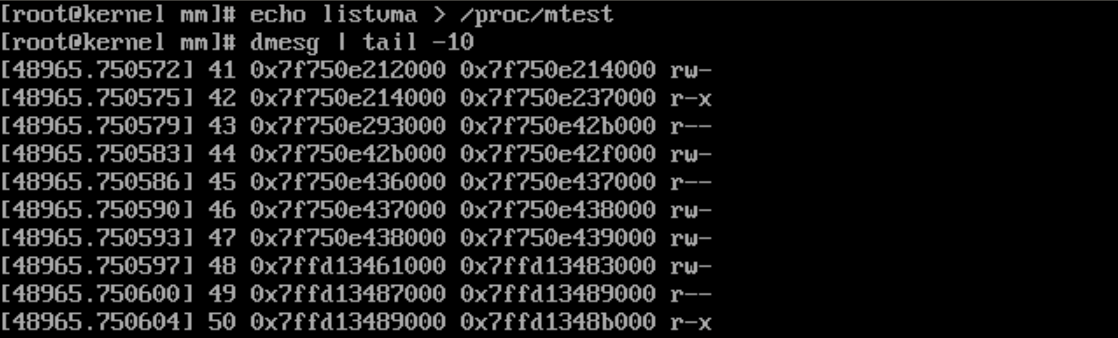
\includegraphics[width=10cm]{listvma.png}
\caption{List virtual memory area}
\end{figure}
\begin{figure}[H]
\centering
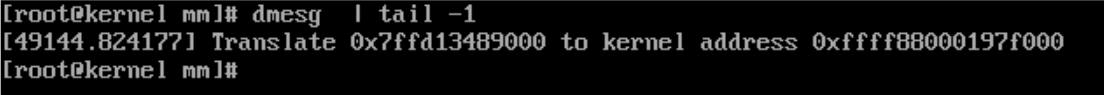
\includegraphics[width=10cm]{findpage.png}
\caption{Find virtual memory page}
\end{figure}
\begin{figure}[H]
\centering
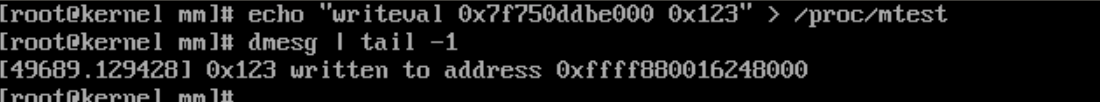
\includegraphics[width=10cm]{writeval.png}
\caption{Write to virtual memory address}
\end{figure}

\section{Conclusion}
In this project, I really leaned a lot about Linux kernel memory management subsystem and a lot about Linux kernel programming APIs. I find memory management is extremely important for model operating systems and I will learn more about this in my free time.




\section*{Acknowledgement}
Thanks Prof. Chen for guidance on Linux kernel and TAs for their hard work.
\end{document}
